\documentclass{beamer}

\usepackage[utf8]{inputenc}
\usepackage[T1]{fontenc}
\usepackage[brazil]{babel}
\usepackage{amsmath, amsfonts, amssymb}
\usepackage{siunitx}
\usepackage{graphicx}
\usepackage{booktabs}
\usepackage{hyperref}

% Estilo SINTEF/XMU copiado para esta pasta
\usepackage{sintefcolor}
\usepackage{beamerthemesintef}
\usefonttheme[onlymath]{serif}
\usetheme{sintef}

% Fundo do título usando os assets locais
\titlebackground*{XMU-assets/XMU-logo-negative.png}

% Caminhos de imagens do TCC
\graphicspath{{../src/Cap03/}{../src/Cap03/imagens/}{../src/Cap03/img/}}

\title[Controle determinístico para CNC]{Controle determinístico para CNC baseado em STM32L475\\com DDA de alta frequência}
\author[Valdir Dias Silva Junior]{Valdir Dias Silva Junior}
\institute{%
  Trabalho de Conclusão de Curso\\[0.2em]
  \small Maceió -- Alagoas
}
\date{Novembro de 2024}

\begin{document}

\maketitle

%--------------------------------------------------------------------
\begin{frame}{Roteiro}
  \tableofcontents
\end{frame}

%====================================================================
\section{Protocolo de comunicação}

%--------------------------------------------------------------------
\begin{frame}{Visão geral do enlace}
  \begin{itemize}
    \item Arquitetura híbrida: Raspberry Pi como mestre de alto nível e STM32L475 como controlador em tempo real.
    \item Comunicação principal via SPI1 (STM32 em modo escravo com DMA circular).
    \item USART1 usada como console de depuração, telemetria e logs de eventos.
    \item Drivers TMC5160 configurados por SPI dedicado e monitorados por registradores de status.
  \end{itemize}
\end{frame}

%--------------------------------------------------------------------
\begin{frame}{Quadro SPI -- Raspberry Pi $\leftrightarrow$ STM32}
  \begin{itemize}
    \item Quadros de \textbf{tamanho fixo}: 42~bytes em modo \emph{full-duplex}.
    \item Estrutura típica:
      \begin{itemize}
        \item \textbf{SOF} (0xAB), \textbf{CMD}, \textbf{FLAGS}, \textbf{LEN}.
        \item \textbf{PAYLOAD} com até 34~bytes úteis.
        \item \textbf{CRC16} sobre os bytes 0..37.
        \item \textbf{EOF} (0x54) como marcador de fim de quadro.
      \end{itemize}
    \item Quando não há resposta pronta, o escravo devolve padrão 0xA5 em todo o payload.
    \item Protocolo baseado em \emph{poll}: o mestre envia pedidos periódicos até receber uma resposta válida.
  \end{itemize}
\end{frame}

%--------------------------------------------------------------------
\begin{frame}{Serviços SPI: LED e Movimento}
  \begin{block}{Serviço LED (\texttt{CMD = 0x10})}
    \begin{itemize}
      \item Requisição: identifica o LED e o modo (\texttt{OFF}, \texttt{ON}, \texttt{TOGGLE}).
      \item Resposta: campo \texttt{STATUS} (OK/erro) e \texttt{LED\_STATE} final.
      \item Exemplo simples para validar integridade do enlace e CRC.
    \end{itemize}
  \end{block}
  \vspace{0.4em}
  \begin{block}{Serviço Movimento (\texttt{CMD = 0x20})}
    \begin{itemize}
      \item Requisição recebe \texttt{AXIS\_MASK}, deslocamentos relativos em passos (X,Y,Z) e \texttt{FEED} em passos/s.
      \item Opcionalmente, parâmetro de \emph{jerk} para suavizar aceleração.
      \item Resposta indica \texttt{STATUS} (aceito/ocupado/erro) e \texttt{QUEUE\_DEPTH} da fila de movimentos.
    \end{itemize}
  \end{block}
\end{frame}

%--------------------------------------------------------------------
\begin{frame}{SPI Raspberry Pi $\leftrightarrow$ TMC5160}
  \begin{itemize}
    \item Transações de 40~bits (5~bytes): 1~byte de endereço + 4~bytes de dados.
    \item Bit mais significativo do endereço define leitura (\textbf{1}) ou escrita (\textbf{0}).
    \item Latência de uma transação: dados lidos em \texttt{SDO} correspondem ao comando anterior.
    \item Utilizado para:
      \begin{itemize}
        \item Programar microstepping, correntes, modo de \emph{chopper} e interpolação (\emph{MicroPlyer}).
        \item Ler \texttt{DRV\_STATUS} e outros registradores de diagnóstico.
      \end{itemize}
  \end{itemize}
\end{frame}

%--------------------------------------------------------------------
\begin{frame}{Fluxo do comando \texttt{cnc-cli}}
  \begin{itemize}
    \item Cliente em Python (\texttt{cnc\_cli.py}) executa uma sequência declarativa em JSON.
    \item Passos incluem:
      \begin{itemize}
        \item Aplicação de \emph{patches} TMC5160 (corrente, microsteps, interpolação).
        \item Atualização de ganhos PID inteiros por eixo.
        \item Enfileiramento de movimentos relativos para o STM32.
      \end{itemize}
    \item Cada comando é validado contra limites de \texttt{application.cfg}; violações abortam a sequência.
    \item Durante o movimento, o cliente monitora erros graves do TMC5160 e aciona medidas de segurança.
  \end{itemize}
\end{frame}

%====================================================================
\section{Arquitetura de hardware}

%--------------------------------------------------------------------
\begin{frame}{Blocos de hardware}
  \begin{itemize}
    \item \textbf{Lógica}: placa STM32L475 operando a \SI{3.3}{V}, com interfaces SPI, USART e GPIO.
    \item \textbf{Drivers de eixo}: módulos com TMC5160 comandados por sinais \texttt{STEP}/\texttt{DIR}/\texttt{EN}.
    \item \textbf{Realimentação}: encoder óptico incremental TMCS-28 (ABN, TTL \SI{5}{V}) acoplado ao eixo.
    \item \textbf{Alimentação}: trilha de \SI{5}{V} para lógica/sensores e alimentação separada filtrada para potência.
    \item \textbf{Segurança}: entradas de E-STOP e sensores de fim de curso integradas ao NVIC com alta prioridade.
  \end{itemize}
\end{frame}

%--------------------------------------------------------------------
\begin{frame}{Layout do controlador CNC}
  \centering
  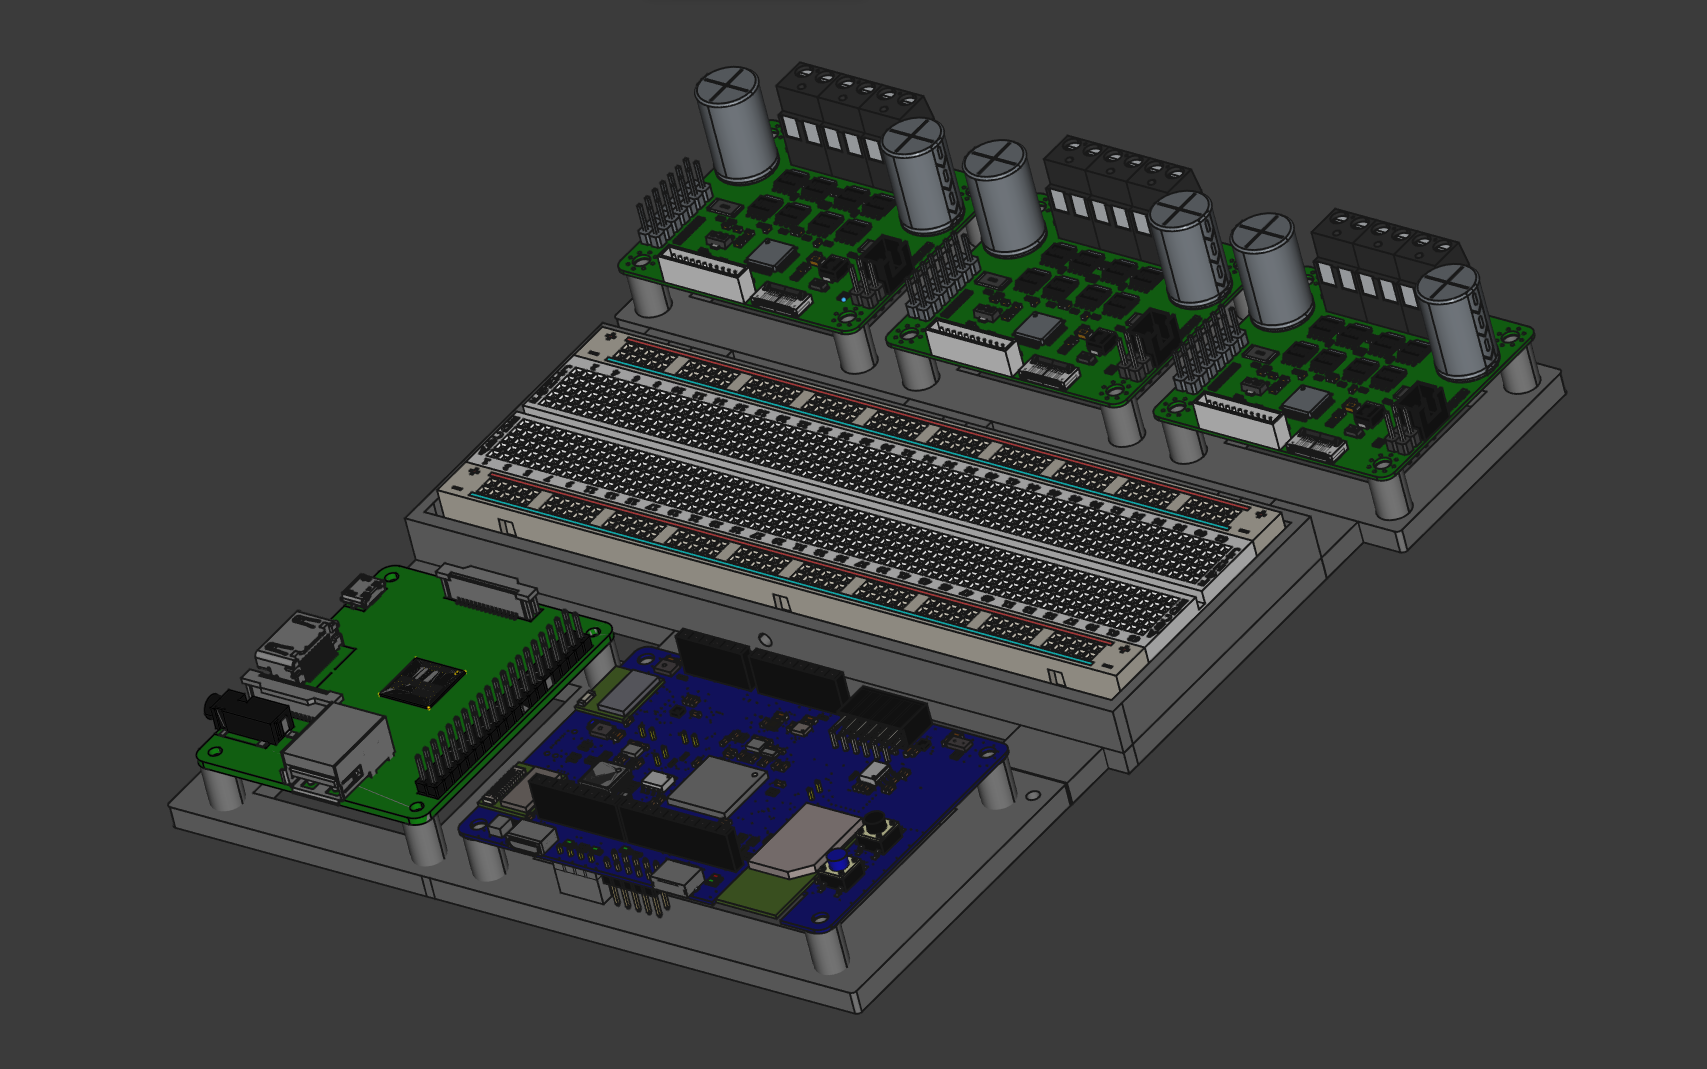
\includegraphics[width=0.75\linewidth]{TCC_CIRCUITO_CONTROLE_COMPLETO.png}
  \vspace{0.5em}

  \small Modelo 3D do controlador CNC com placa STM32, interface para Raspberry Pi,
  base de prototipagem e módulos de potência TMC5160.
\end{frame}

%--------------------------------------------------------------------
\begin{frame}{Vista superior do conjunto}
  \centering
  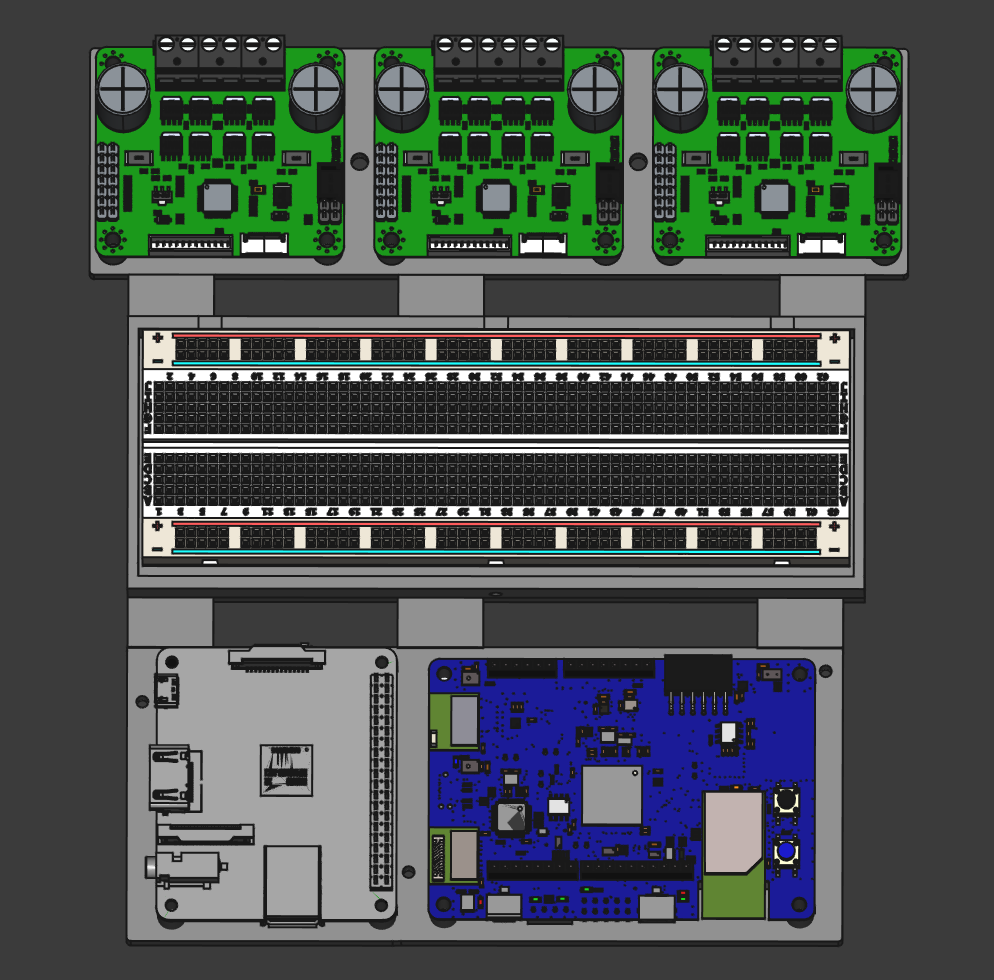
\includegraphics[width=0.75\linewidth]{TCC_CIRCUITO_CONTROLE_SEMFAN_CIMA.png}
  \vspace{0.5em}

  \small Vista superior destacando a distribuição das placas e o roteamento
  entre lógica, drivers e sensores.
\end{frame}

%--------------------------------------------------------------------
\begin{frame}{Encoder óptico TMCS-28}
  \begin{itemize}
    \item Encoder incremental TMCS-28-10k com resolução efetiva de 40\,000 contagens por volta.
    \item Saídas A/B/N em TTL \SI{5}{V}, condicionadas para \SI{3.3}{V} antes de chegar ao STM32.
    \item Canais A/B ligados a TIM3, LPTIM1 e TIM5 em modo \emph{encoder}, liberando a CPU de interrupções.
    \item Canal N utilizado como referência de índice na rotina de \emph{homing}.
  \end{itemize}
\end{frame}

%====================================================================
\section{Arquitetura de software}

%--------------------------------------------------------------------
\begin{frame}{Camadas do firmware}
  \begin{itemize}
    \item \textbf{Core}:
      \begin{itemize}
        \item Código gerado pelo STM32CubeMX (HAL, inicialização de clock, GPIO, timers, SPI, USART).
      \end{itemize}
    \item \textbf{App}:
      \begin{itemize}
        \item Laço principal \texttt{app\_poll}, agendador de serviços e integração com filas SPI/USART.
      \end{itemize}
    \item \textbf{Services}:
      \begin{itemize}
        \item Gerador de passos, controle PID, serviço de homing, serviço de movimento e roteador de mensagens.
      \end{itemize}
  \end{itemize}
\end{frame}

%--------------------------------------------------------------------
\begin{frame}{Pipeline SPI no firmware}
  \begin{itemize}
    \item SPI1 configurado como escravo com DMA circular recebendo quadros de 42~bytes.
    \item Cada \emph{poll} do mestre:
      \begin{itemize}
        \item Congela temporariamente o DMA para permitir processamento de comando em \texttt{app\_poll}.
        \item Se houver resposta pronta, o payload é promovido para o buffer ativo do DMA.
      \end{itemize}
    \item Caso contrário, o mestre recebe quadro com padrão 0xA5 e repete o \emph{poll}.
    \item Parâmetro \texttt{APP\_SPI\_RESTART\_DEFER\_MAX} ajusta o número máximo de tentativas antes de \emph{fallback}.
  \end{itemize}
\end{frame}

%--------------------------------------------------------------------
\begin{frame}{Roteiro incremental de inicialização}
  \begin{itemize}
    \item Configuração do clock principal para \SI{80}{\mega\hertz}.
    \item Definição de prioridades no NVIC: E-STOP, TIM6, SPI1/DMA, TIM7, USART1.
    \item Calibração dos temporizadores:
      \begin{itemize}
        \item TIM6 @ 50~kHz para geração de \emph{STEP}.
        \item TIM7 @ 1~kHz para rampas, leitura de encoders e controle.
      \end{itemize}
    \item Inicialização do SPI1 com DMA circular e integração com o serviço SPI.
    \item Integração da USART1 como console de log não bloqueante.
  \end{itemize}
\end{frame}

%====================================================================
\section{Controle de movimento}

%--------------------------------------------------------------------
\begin{frame}{Temporizadores e DDA}
  \begin{itemize}
    \item TIM6 configurado com $PSC = 79$ e $ARR = 19$, resultando em \SI{50}{\kilo\hertz}.
    \item Cada tick de \SI{20}{\micro\second} alimenta o DDA em ponto fixo para geração de \emph{STEP}.
    \item TIM7 configurado para \SI{1}{\kilo\hertz}, responsável por:
      \begin{itemize}
        \item Cálculo de rampas trapezoidais (aceleração/desaceleração).
        \item Leitura dos contadores de encoder e atualização dos erros.
        \item Aplicação do controle PI/PD de posição/velocidade.
      \end{itemize}
  \end{itemize}
\end{frame}

%--------------------------------------------------------------------
\begin{frame}{DDA: geração de passos determinística}
  \centering
  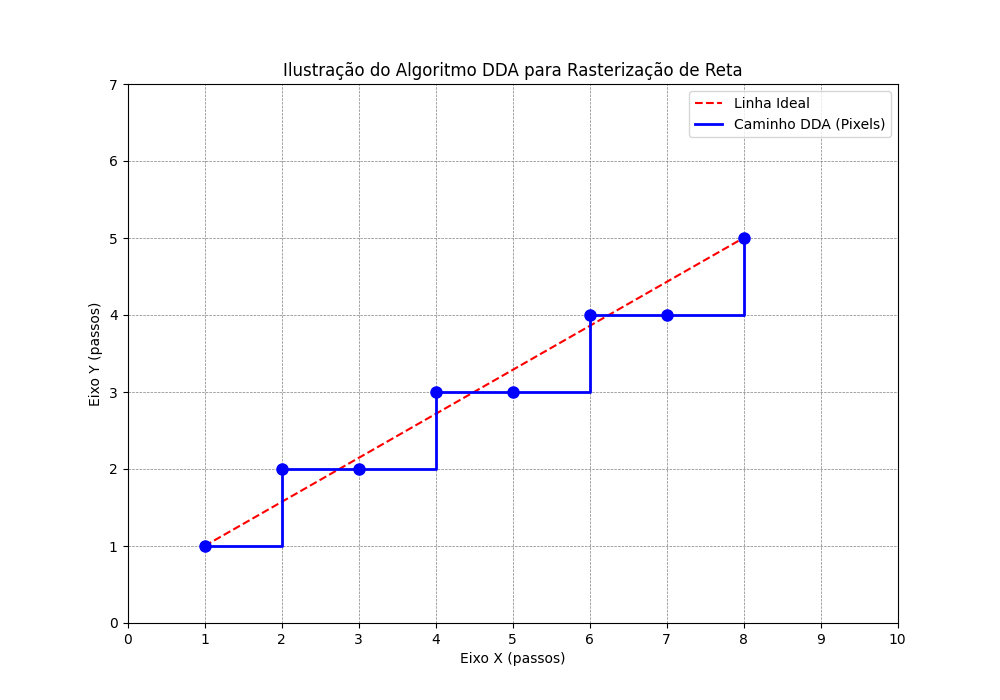
\includegraphics[width=0.75\linewidth]{dda_line_rasterization.png}
  \vspace{0.5em}

  \small O DDA acumula erro fracionário a cada tick de TIM6 e gera pulsos
  \emph{STEP} quando o limiar é ultrapassado, aproximando trajetórias contínuas
  por incrementos discretos sincronizados entre eixos.
\end{frame}

%--------------------------------------------------------------------
\begin{frame}{Compatibilidade com o TMC5160 (STEP/DIR)}
  \begin{itemize}
    \item Datasheet do TMC5160 impõe tempos mínimos de pulso na ordem de dezenas de ns.
    \item Projeto utiliza:
      \begin{itemize}
        \item $t_{SH} = t_{SL} = \SI{20}{\micro\second}$ para largura alta e baixa de \emph{STEP}.
        \item $t_{DSU} = \SI{20}{\micro\second}$ entre mudança em \emph{DIR} e próximo \emph{STEP}.
        \item Tempo de assentamento de ENABLE de \SI{40}{\micro\second}.
      \end{itemize}
    \item Margens de segurança de várias ordens de grandeza em relação às especificações.
  \end{itemize}
\end{frame}

%--------------------------------------------------------------------
\begin{frame}{Comparação de pulsos STEP}
  \centering
  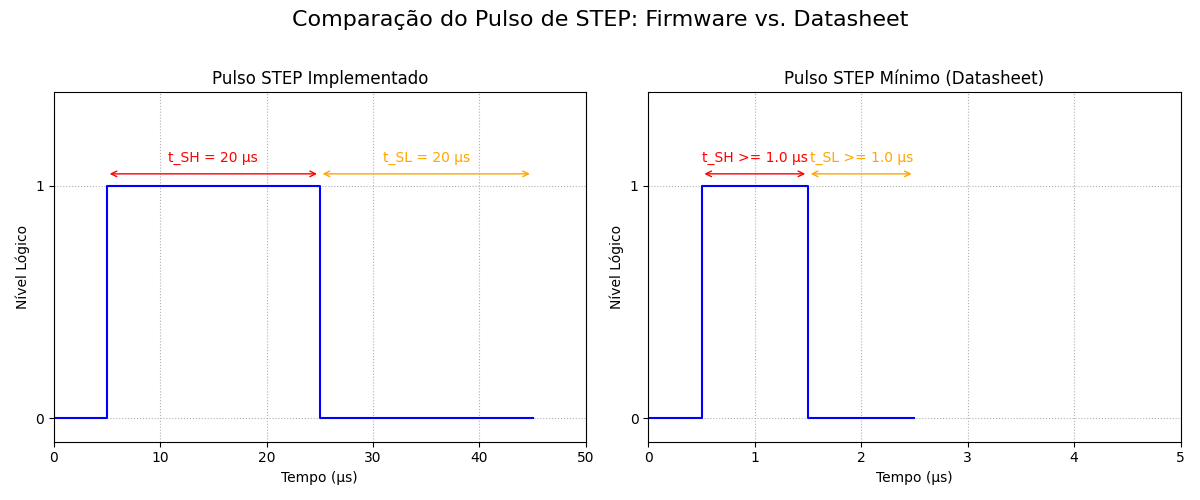
\includegraphics[width=0.85\linewidth]{step_pulse_comparison.png}
  \vspace{0.5em}

  \small Pulso de \emph{STEP} implementado no firmware (esquerda) comparado ao
  pulso mínimo requerido pelo TMC5160 (direita), evidenciando ampla margem temporal.
\end{frame}

%--------------------------------------------------------------------
\begin{frame}{Malhas de posição e velocidade}
  \begin{itemize}
    \item Encoders em modo quadratura fornecem posição incremental precisa para cada eixo.
    \item Laço em \SI{1}{\kilo\hertz} calcula:
      \begin{itemize}
        \item Erro de posição entre referência (trajetória do DDA) e leitura do encoder.
        \item Erro de velocidade derivado das contagens por janela de tempo.
      \end{itemize}
    \item Controladores PI/PD com ganhos inteiros garantem rastreamento estável e limitam sobre-elevação.
    \item Supervisão de sincronização cruzada entre eixos (\emph{cross-coupled control}).
  \end{itemize}
\end{frame}

%--------------------------------------------------------------------
\begin{frame}{Modelo FOPDT e síntese de ganhos PD}
  \begin{itemize}
    \item Malha de velocidade aproximada por modelo FOPDT: ganho $K$, tempo morto $L$ e constante de tempo $\tau$.
    \item Parâmetros identificados a partir de respostas a degrau de velocidade obtidas via telemetria.
    \item Ganhos PD contínuos sintetizados por regras de Ziegler--Nichols para curva de reação.
    \item Ganhos contínuos escalonados para formato inteiro (fator de escala $S=256$) e catalogados por eixo/microstep.
  \end{itemize}
\end{frame}

%--------------------------------------------------------------------
\begin{frame}{Validação do modelo FOPDT}
  \centering
  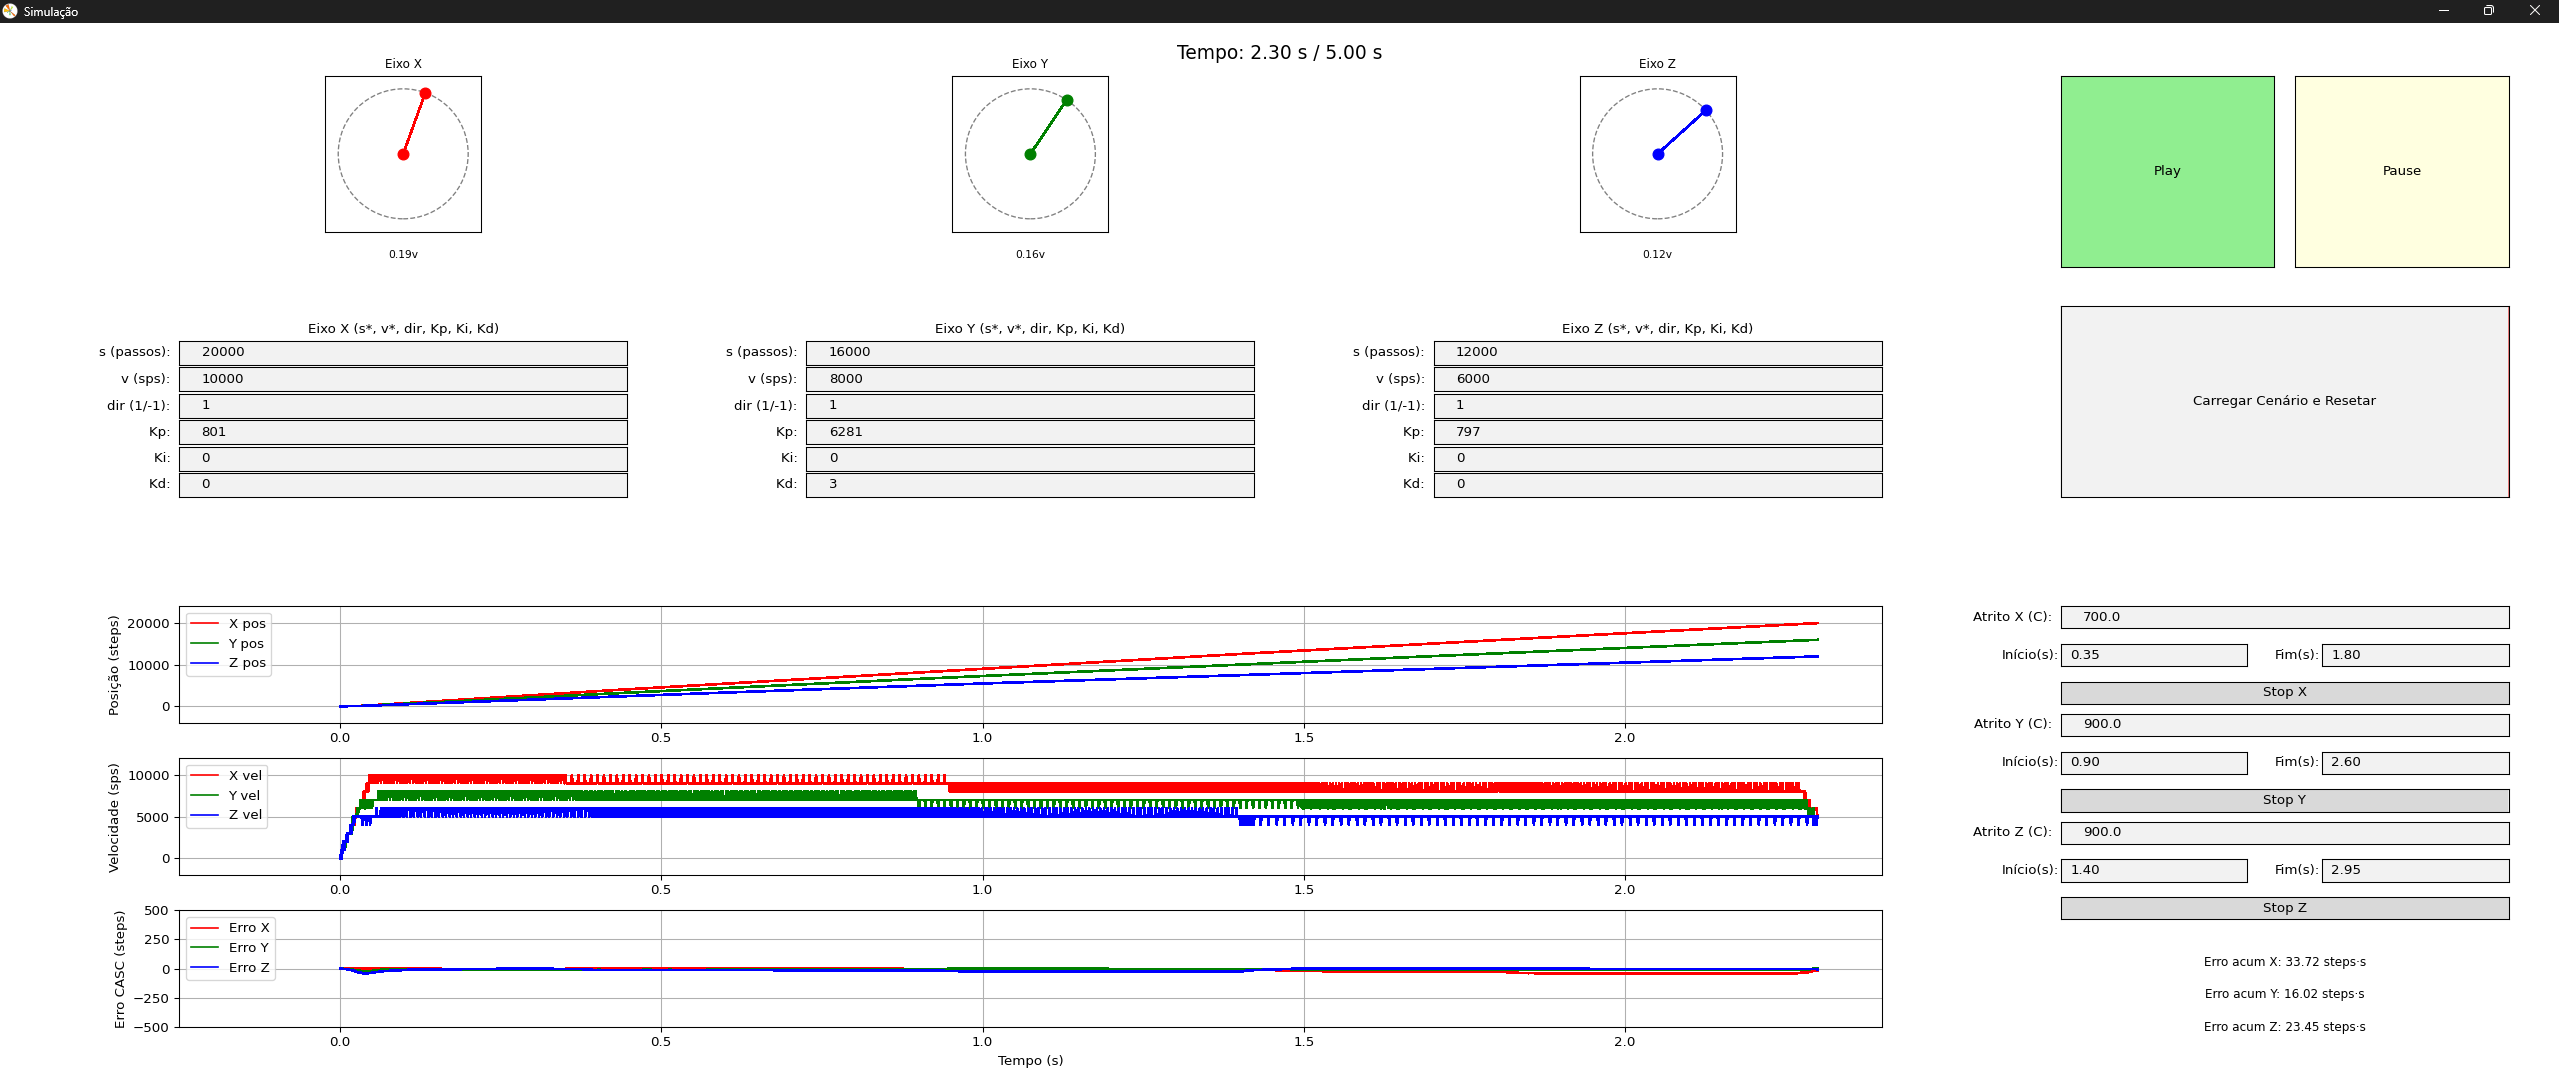
\includegraphics[width=0.85\linewidth]{SimulacaoTCC.png}
  \vspace{0.5em}

  \small Sobreposição entre velocidade medida e resposta teórica do modelo FOPDT,
  mostrando boa aderência na faixa de operação de interesse para os três eixos.
\end{frame}

%====================================================================
\section{Resultados e conclusão}

%--------------------------------------------------------------------
\begin{frame}{Desempenho dos serviços principais}
  \begin{itemize}
    \item Gerador de passos (TIM6) opera próximo de \SI{50}{\kilo\hertz} com variação pequena entre ciclos.
    \item Laço de controle (TIM7) apresenta \emph{jitter} na ordem de poucos \si{\micro\second}.
    \item Pipeline SPI confirma necessidade de 2--3 \emph{polls} para entrega de respostas completas.
    \item Otimização de promoção direta de payload ao buffer de DMA reduziu o tempo médio entre \emph{polls}.
  \end{itemize}
\end{frame}

%--------------------------------------------------------------------
\begin{frame}{Comparação simulação vs experimento}
  \centering
  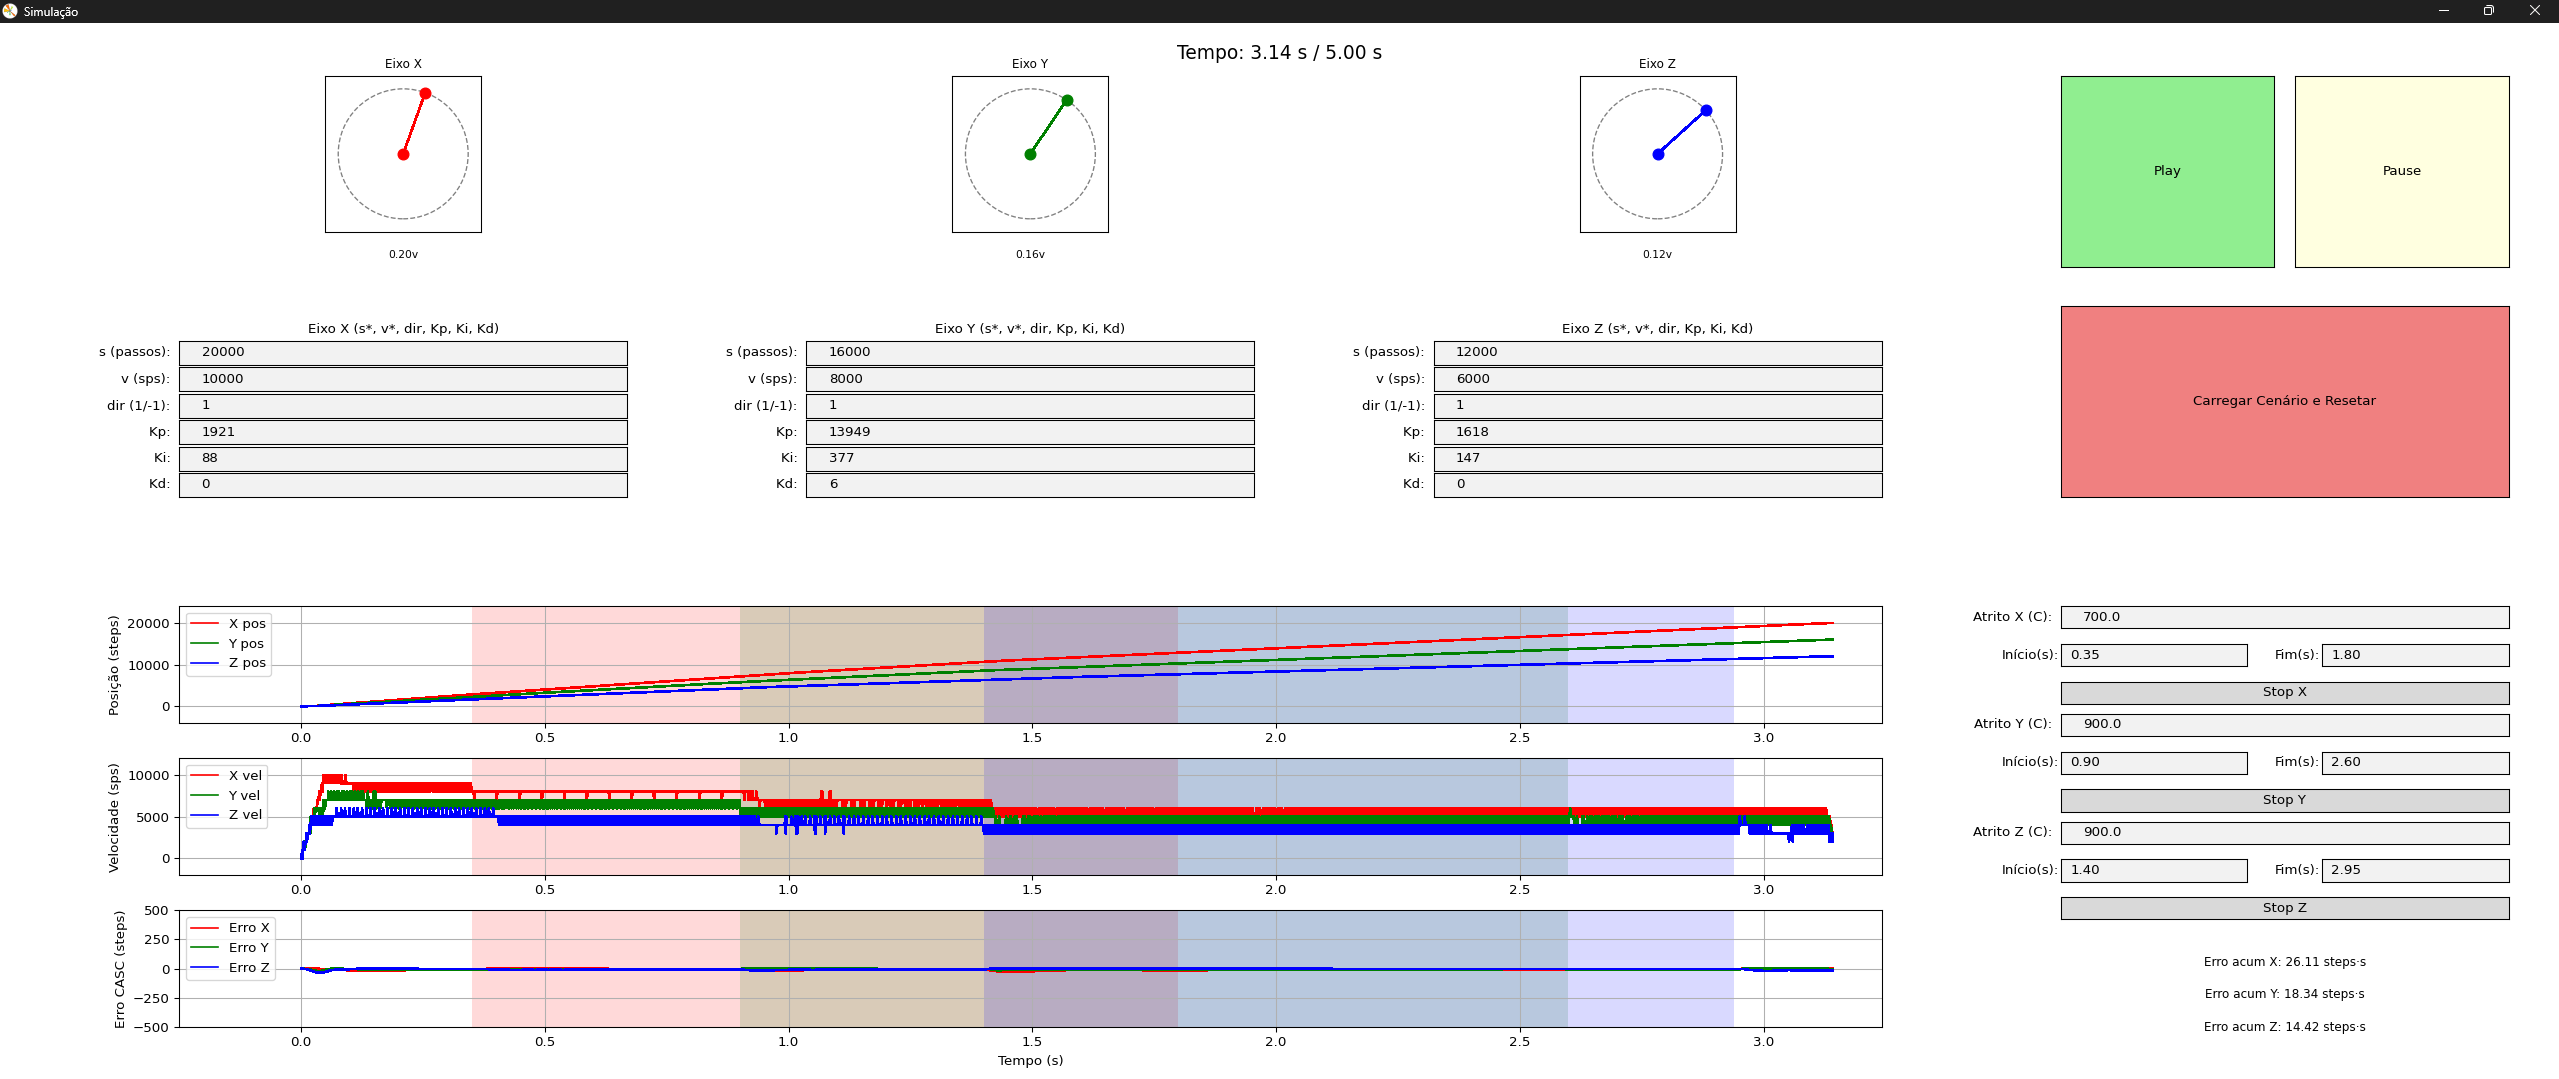
\includegraphics[width=0.9\linewidth]{TCC_SIMULACAO_COM_ATRITO.png}
  \vspace{0.5em}

  \small Comparação entre velocidades de passo medidas e simuladas sob carga:
  boa coerência geral, com desvios explicados por atrito e assimetrias de carga entre eixos.
\end{frame}

%--------------------------------------------------------------------
\begin{frame}{Conclusões}
  \begin{itemize}
    \item Controlador CNC embarcado em STM32L475 atinge geração determinística de pulsos e malhas de controle estáveis.
    \item Protocolo SPI com quadros fixos e CRC16 garante comunicação robusta com a Raspberry Pi.
    \item Metodologia incremental facilitou a validação de cada bloco crítico (timers, SPI, encoders, PID).
    \item Identificação FOPDT e catálogo de ganhos PD proporcionam sintonia sistemática da malha de velocidade.
  \end{itemize}
\end{frame}

%--------------------------------------------------------------------
\begin{frame}{Trabalhos futuros}
  \begin{itemize}
    \item Reduzir a dependência de múltiplos \emph{polls} SPI por comando.
    \item Explorar reinicialização imediata do DMA assim que uma resposta estiver disponível.
    \item Investigar perfis de movimento mais agressivos com prescalers adaptativos.
    \item Avaliar envio de múltiplos comandos por ciclo SPI para melhor aproveitamento do canal.
  \end{itemize}
\end{frame}

%--------------------------------------------------------------------
\begin{frame}[plain]
  \centering
  \vfill
  {\LARGE Obrigado!}\\[1em]
  \large Perguntas?
  \vfill
\end{frame}

\end{document}
